\documentclass{beamer}
\usepackage{../../shared/styles/custom}
\usepackage{../../shared/styles/conventions}

\usepackage{grffile}

\title{Lasso Regression}
\date{\today}
\author{Nipun Batra}
\institute{IIT Gandhinagar}
\begin{document}
  \maketitle
  
\begin{frame}{Outline}
\tableofcontents
\end{frame}

\section{Introduction and Motivation}

\begin{frame}{What is Lasso Regression?}
\begin{definitionbox}{LASSO}
\textbf{L}east \textbf{A}bsolute \textbf{S}hrinkage and \textbf{S}election \textbf{O}perator
\end{definitionbox}
\pause

\begin{keypointsbox}{Key Properties}
\begin{itemize}
\item Uses L1 penalty (absolute values) instead of L2 penalty
\item Leads to \textbf{sparse solutions} (many coefficients become exactly zero)
\item Performs automatic feature selection
\item Popular for high-dimensional problems
\end{itemize}
\end{keypointsbox}
\end{frame}

\section{Mathematical Formulation}

\begin{frame}{Problem: Why Not Just Use Ridge?}
\begin{alertbox}{Limitation of Ridge Regression}
Ridge regression shrinks coefficients but \textbf{never makes them exactly zero}
\end{alertbox}
\pause

\begin{examplebox}{High-Dimensional Problem}
\begin{itemize}
\item 1000 features, only 50 are truly relevant
\item Ridge gives tiny but non-zero coefficients for irrelevant features
\item Model is not interpretable
\item Need automatic feature selection!
\end{itemize}
\end{examplebox}
\end{frame}

\begin{frame}{Lasso Objective Function}
\begin{definitionbox}{Constrained Form}
$$\vtheta_{\text{opt}} = \argmin_{\vtheta} \|(\vy-\mX\vtheta)\|_2^2 \text{ subject to } \|\vtheta\|_1 \leq s$$
\end{definitionbox}
\pause

\begin{theorembox}{Penalized Form (Using Lagrangian Duality)}
Constrained form is equivalent to:
$$\vtheta_{\text{opt}} = \argmin_{\vtheta} \underbrace{\|(\vy-\mX\vtheta)\|_2^2 + \lambda \|\vtheta\|_1}_{\text{Lasso Objective}}$$
\end{theorembox}
\pause

\begin{codebox}{L1 Norm (Manhattan Distance)}
$$\|\vtheta\|_1 = |\theta_1| + |\theta_2| + \cdots + |\theta_d| = \sum_{j=1}^d |\theta_j|$$
\end{codebox}
\end{frame}

\begin{frame}{The Challenge: Non-Differentiability}
\begin{alertbox}{Problem}
The L1 norm $\|\vtheta\|_1 = \sum_j |\theta_j|$ is \textbf{not differentiable} at $\theta_j = 0$
\end{alertbox}
\pause

\begin{codebox}{Cannot Use Standard Calculus}
$$\frac{\partial}{\partial \vtheta} \left[ \|(\vy-\mX\vtheta)\|_2^2 + \lambda \|\vtheta\|_1 \right] = 0$$
This fails because $\frac{\partial |\theta_j|}{\partial \theta_j}$ is undefined at $\theta_j = 0$
\end{codebox}

\begin{keypointsbox}{Solution Approaches}
{\small
\begin{itemize}
\item \textbf{Coordinate Descent}: Optimize one coefficient at a time
\item \textbf{Subgradient Methods}: Generalize derivatives to non-smooth functions
\end{itemize}
}
\end{keypointsbox}
\end{frame}

\section{Why Lasso Gives Sparsity}

\begin{frame}{Sparsity: The Key Question}
\begin{alertbox}{Central Question}
Why does Lasso produce sparse solutions while Ridge doesn't?
\end{alertbox}
\pause

\begin{keypointsbox}{Two Perspectives}
\begin{itemize}
\item \textbf{Geometric}: Shape of constraint regions
\item \textbf{Algorithmic}: Behavior of optimization algorithms
\end{itemize}
\end{keypointsbox}
\pause

\begin{examplebox}{Preview}
We'll see why $L_p$ norms with $p < 2$ promote sparsity
\end{examplebox}
\end{frame}

\subsection{Geometric Interpretation}

\begin{frame}{L2 Norm: Ridge Constraint}
\begin{columns}
\begin{column}{0.6\textwidth}
\begin{center}
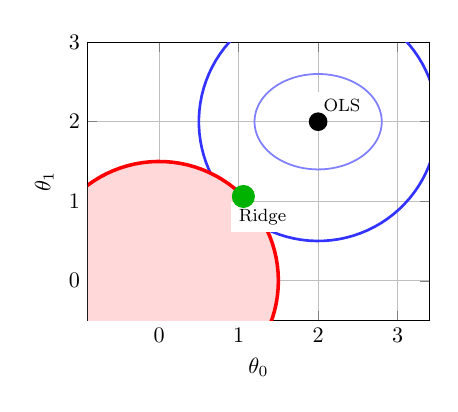
\begin{tikzpicture}[scale=0.8]
\begin{axis}[
    width=7cm, height=6cm,
    xlabel={$\theta_0$}, ylabel={$\theta_1$},
    xmin=-0.5, xmax=3, ymin=-0.5, ymax=3,
    axis equal, grid=major
]
% OLS solution
\addplot[only marks, mark=*, mark size=4pt, color=black] coordinates {(2, 2)};
\node[fill=white] at (axis cs:2.3,2.2) {\footnotesize OLS};
% RSS ellipses
\addplot[domain=0:360, samples=100, thick, blue!50] ({0.8*cos(x) + 2}, {0.6*sin(x) + 2});
\addplot[domain=0:360, samples=100, very thick, blue!80] ({1.5*cos(x) + 2}, {1.5*sin(x) + 2});
% L2 constraint circle
\addplot[domain=0:360, samples=100, ultra thick, red, fill=red!15] ({1.5*cos(x)}, {1.5*sin(x)});
% Ridge solution
\addplot[only marks, mark=*, mark size=5pt, color=green!70!black] coordinates {(1.06, 1.06)};
\node[fill=white] at (axis cs:1.3,0.8) {\footnotesize Ridge};
\end{axis}
\end{tikzpicture}
\end{center}
\end{column}

\begin{column}{0.4\textwidth}
\begin{keypointsbox}{L2 Properties}
\begin{itemize}
\item \textbf{Shape}: Perfect circle
\item \textbf{Constraint}: $\theta_0^2 + \theta_1^2 \leq c$
\item \textbf{Boundary}: Smooth everywhere
\item \textbf{Intersection}: Rarely on axes
\item \textbf{Result}: No sparsity
\end{itemize}
\end{keypointsbox}

\begin{alertbox}{Key Issue}
Ridge shrinks coefficients but never makes them exactly zero
\end{alertbox}
\end{column}
\end{columns}
\end{frame}

\begin{frame}{L1 Norm: Lasso Constraint}
\begin{columns}
\begin{column}{0.6\textwidth}
\begin{center}
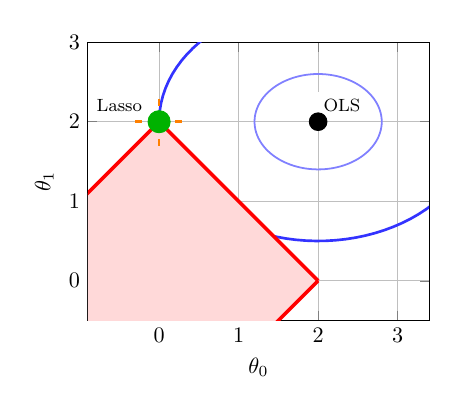
\begin{tikzpicture}[scale=0.8]
\begin{axis}[
    width=7cm, height=6cm,
    xlabel={$\theta_0$}, ylabel={$\theta_1$},
    xmin=-0.5, xmax=3, ymin=-0.5, ymax=3,
    axis equal, grid=major
]
% OLS solution
\addplot[only marks, mark=*, mark size=4pt, color=black] coordinates {(2, 2)};
\node[fill=white] at (axis cs:2.3,2.2) {\footnotesize OLS};
% RSS ellipses
\addplot[domain=0:360, samples=100, thick, blue!50] ({0.8*cos(x) + 2}, {0.6*sin(x) + 2});
\addplot[domain=0:360, samples=100, very thick, blue!80] ({2*cos(x) + 2}, {1.5*sin(x) + 2});
% L1 constraint diamond
\addplot[ultra thick, red, fill=red!15] coordinates {(2,0) (0,2) (-2,0) (0,-2) (2,0)};
% Lasso solution at corner
\addplot[only marks, mark=*, mark size=5pt, color=green!70!black] coordinates {(0, 2)};
\node[fill=white] at (axis cs:-0.5,2.2) {\footnotesize Lasso};
% Highlight corner
\draw[very thick, orange, dashed] (-0.3,2) -- (0.3,2);
\draw[very thick, orange, dashed] (0,1.7) -- (0,2.3);
\end{axis}
\end{tikzpicture}
\end{center}
\end{column}

\begin{column}{0.4\textwidth}
\begin{keypointsbox}{L1 Properties}
\begin{itemize}
\item \textbf{Shape}: Diamond/rhombus
\item \textbf{Constraint}: $|\theta_0| + |\theta_1| \leq c$
\item \textbf{Corners}: Sharp at axes
\item \textbf{Intersection}: High probability on axes
\item \textbf{Result}: Automatic sparsity!
\end{itemize}
\end{keypointsbox}

\begin{theorembox}{Sparsity Mechanism}
Sharp corners at axes $\Rightarrow$ solutions with $\theta_0 = 0$ or $\theta_1 = 0$
\end{theorembox}
\end{column}
\end{columns}
\end{frame}

\begin{frame}{$L_p$ Norm: Even More Sparsity ($p < 1$)}
\begin{columns}
\begin{column}{0.6\textwidth}
\begin{center}
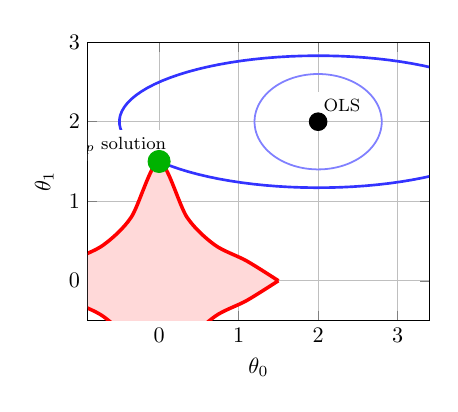
\begin{tikzpicture}[scale=0.8]
\begin{axis}[
    width=7cm, height=6cm,
    xlabel={$\theta_0$}, ylabel={$\theta_1$},
    xmin=-0.5, xmax=3, ymin=-0.5, ymax=3,
    axis equal, grid=major
]
% OLS solution
\addplot[only marks, mark=*, mark size=4pt, color=black] coordinates {(2, 2)};
\node[fill=white] at (axis cs:2.3,2.2) {\footnotesize OLS};
% RSS ellipses
\addplot[domain=0:360, samples=100, thick, blue!50] ({0.8*cos(x) + 2}, {0.6*sin(x) + 2});
\addplot[domain=0:360, samples=100, very thick, blue!80] ({2.5*cos(x) + 2}, {0.83*sin(x) + 2});
% Lp constraint (concave)
\addplot[ultra thick, red, smooth, fill=red!15] coordinates {
    (1.5,0) (1.1,0.25) (0.7,0.45) (0.35,0.8) (0,1.5)
    (-0.35,0.8) (-0.7,0.45) (-1.1,0.25) (-1.5,0)
    (-1.1,-0.25) (-0.7,-0.45) (-0.35,-0.8) (0,-1.5)
    (0.35,-0.8) (0.7,-0.45) (1.1,-0.25) (1.5,0)
};
% Solution at ultra-sharp corner
\addplot[only marks, mark=*, mark size=5pt, color=green!70!black] coordinates {(0, 1.5)};
\node[fill=white] at (axis cs:-0.5,1.7) {\footnotesize $L_p$ solution};
\end{axis}
\end{tikzpicture}
\end{center}
\end{column}

\begin{column}{0.4\textwidth}
\begin{keypointsbox}{$L_p$ Properties $(p<1)$}
\begin{itemize}
\item \textbf{Shape}: Highly concave
\item \textbf{Constraint}: $(|\theta_0|^p + |\theta_1|^p)^{1/p} \leq c$
\item \textbf{Corners}: Ultra-sharp at axes
\item \textbf{Sparsity}: Extremely high
\item \textbf{Problem}: Non-convex!
\end{itemize}
\end{keypointsbox}

\begin{alertbox}{Trade-off}
Better sparsity but computational difficulty (non-convex optimization)
\end{alertbox}
\end{column}
\end{columns}
\end{frame}

\begin{frame}{Sparsity Progression: $L_2 \to L_1 \to L_p$}
\begin{theorembox}{Key Insight}
As $p$ decreases from 2 to 1 to $p < 1$:
\begin{itemize}
\item Constraint regions become more \textbf{pointed} at axes
\item Probability of intersection at axes \textbf{increases}
\item Sparsity \textbf{increases}
\item Optimization difficulty \textbf{increases}
\end{itemize}
\end{theorembox}

\begin{examplebox}{Why $p = 1$ is Special}
\begin{itemize}
\item Still promotes sparsity (sharp corners)
\item Remains convex (unlike $p < 1$) and Computationally tractable
\item Perfect balance of sparsity and solvability
\end{itemize}
\end{examplebox}
\end{frame}

\subsection{Gradient Descent Interpretation}

\begin{frame}{L2 vs L1: Gradient Behavior}
\begin{columns}
\begin{column}{0.5\textwidth}
\begin{keypointsbox}{L2 Penalty: $f(\theta) = \frac{1}{2}\theta^2$}
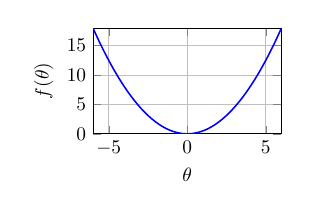
\begin{tikzpicture}[scale=0.7]
\begin{axis}[
    width=5cm, height=3.5cm,
    xlabel={$\theta$}, ylabel={$f(\theta)$},
    xmin=-6, xmax=6, ymin=0, ymax=18,
    grid=major
]
\addplot[domain=-6:6, samples=100, thick, blue] {0.5*x^2};
\end{axis}
\end{tikzpicture}
\\[0.3em]
{\small Gradient: $\frac{df}{d\theta} = \theta$ \\[0.1em]
Shrinks proportionally to current value}
\end{keypointsbox}
\end{column}


\begin{column}{0.5\textwidth}
\begin{keypointsbox}{L1 Penalty: $f(\theta) = |\theta|$}
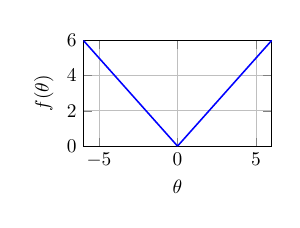
\begin{tikzpicture}[scale=0.7]
\begin{axis}[
    width=5cm, height=3.5cm,
    xlabel={$\theta$}, ylabel={$f(\theta)$},
    xmin=-6, xmax=6, ymin=0, ymax=6,
    grid=major
]
\addplot[domain=-6:0, samples=100, thick, blue] {-x};
\addplot[domain=0:6, samples=100, thick, blue] {x};
\end{axis}
\end{tikzpicture}
\\[0.3em]
{\small Subgradient: $\text{sign}(\theta) = \pm 1$ \\[0.1em]
Constant push toward zero}
\end{keypointsbox}
\end{column}
\end{columns}
\end{frame}

\begin{frame}{L2 vs L1: Gradient Behavior}

\begin{examplebox}{Example: Start at $\theta = 5$}
{\small
\textbf{L2}: $5 \to 2.5 \to 1.25 \to 0.625 \to \ldots$ (never exactly zero) \\[0.1em]
\textbf{L1}: $5 \to 4.5 \to 4.0 \to 3.5 \to \ldots \to 0$ (reaches zero in finite steps)
}
\end{examplebox}
\end{frame}

\section{Geometric Interpretation}

\begin{frame}{Sample Dataset for Demonstration}
\begin{examplebox}{True Function}
We'll demonstrate Lasso on a simple linear relationship: $y = 4x + 7$
\end{examplebox}

\begin{figure}
    \centering
    \includegraphics[width=0.65\linewidth]{../assets/lasso-regression/figures/true_function.pdf}
    \caption{{\footnotesize Sample data from $y = 4x + 7$ with noise}}
    \label{fig:my_label}
\end{figure}
\end{frame}

\begin{frame}{Geometric Interpretation: L1 vs L2 Constraints}
\begin{figure}
    \centering
    \includegraphics[width=0.6\linewidth]{../assets/lasso-regression/figures/lasso_base_contour.pdf}
    \caption{{\footnotesize L1 vs L2 constraint regions}}
    \label{fig:my_label}
\end{figure}

\begin{keypointsbox}{Key Insight}
{\footnotesize
Diamond corners $\Rightarrow$ exact zeros! Circle $\Rightarrow$ no sparsity.
}
\end{keypointsbox}
\end{frame}

\section{Regularization Effects}

\begin{frame}{Effect of $\lambda$ on Solution Path}
\begin{alertbox}{Regularization Parameter}
$\lambda$ controls fit vs sparsity trade-off
\end{alertbox}

\begin{columns}
\begin{column}{0.5\textwidth}
\begin{figure}
\includegraphics[width=\linewidth]{../assets/lasso-regression/figures/lasso_1.0.pdf}
\caption{{\footnotesize $\lambda = 1.0$ - Moderate}}
\end{figure}
\end{column}
\begin{column}{0.5\textwidth}
\begin{figure}
\includegraphics[width=\linewidth]{../assets/lasso-regression/figures/lasso_1.25.pdf}
\caption{{\footnotesize $\lambda = 1.25$ - Higher}}
\end{figure}
\end{column}
\end{columns}
\end{frame}

\begin{frame}{Increasing Regularization Strength}
\begin{columns}
\begin{column}{0.5\textwidth}
\begin{figure}
\includegraphics[width=\linewidth]{../assets/lasso-regression/figures/lasso_1.5.pdf}
\caption{{\footnotesize $\lambda = 1.5$ - Strong}}
\end{figure}
\end{column}
\begin{column}{0.5\textwidth}
\begin{figure}
\includegraphics[width=\linewidth]{../assets/lasso-regression/figures/lasso_2.0.pdf}
\caption{{\footnotesize $\lambda = 2.0$ - Very strong}}
\end{figure}
\end{column}
\end{columns}

\begin{keypointsbox}{Observation}
As $\lambda$ increases $\rightarrow$ more coefficients become exactly zero (automatic feature selection)
\end{keypointsbox}
\end{frame}

\begin{frame}{Lasso Regularization Path}
\begin{figure}
    \centering
    \includegraphics[width=0.6\linewidth]{../assets/lasso-regression/figures/lasso_reg.pdf}
    \caption{{\footnotesize Coefficient values vs $\lambda$}}
    \label{fig:my_label}
\end{figure}

\begin{keypointsbox}{Key Observations}
{\small
\begin{itemize}
\item Coefficients shrink to zero as $\lambda$ increases
\item Natural feature selection ordering
\end{itemize}
}
\end{keypointsbox}
\end{frame}

\section{Feature Selection Properties}

\begin{frame}{Lasso for Automatic Feature Selection}
\begin{definitionbox}{Automatic Feature Selection}
Lasso performs regression and feature selection simultaneously by setting irrelevant coefficients to exactly zero
\end{definitionbox}

\begin{keypointsbox}{Key Advantages}
{\small
\begin{itemize}
\item \textbf{Sparsity}: Many coefficients $\rightarrow$ exactly zero
\item \textbf{Interpretability}: Understand which features matter
\item \textbf{Efficiency}: Fewer parameters, faster prediction
\end{itemize}
}
\end{keypointsbox}

\end{frame}

\section{Subgradient Methods}

\begin{frame}{What is a Subgradient?}
A subgradient generalizes the concept of gradient to convex but non-differentiable functions
\pause

\begin{examplebox}{Classic Example}
    \small{
For $f(x) = |x|$:
\begin{itemize}
\item $f'(x) = 1$ when $x > 0$
\item $f'(x) = -1$ when $x < 0$  
\item $f'(0)$ is undefined, but subgradient $\in [-1, 1]$
\end{itemize}}
\end{examplebox}
\pause

\small{
\begin{alertbox}{Why Important for Lasso?}
The L1 penalty $|\theta_j|$ is non-differentiable at $\theta_j = 0$
\end{alertbox}
}
\end{frame}

\begin{frame}{Subgradient: Visual Intuition}
\begin{columns}
\begin{column}{0.6\textwidth}
\begin{figure}
\centering
\includegraphics[width=\linewidth]{../assets/lasso-regression/diagrams/subgradient_1.jpg}
\caption{{\footnotesize Non-differentiable function at $x_0$}}
\label{fig:Non-differentiable function}
\end{figure}
\end{column}
\begin{column}{0.4\textwidth}
\begin{alertbox}{Task}
Find the "derivative" of $f(x)$ at the non-differentiable point $x = x_0$
\end{alertbox}

\begin{codebox}{Construction}
Find differentiable $g(x)$ such that:
\begin{itemize}
\item $g(x_0) = f(x_0)$
\item $g(x) \leq f(x)$ for all $x$
\end{itemize}
\end{codebox}
\end{column}
\end{columns}
\end{frame}

\begin{frame}{Subgradient of $|x|$ at $x = 0$}
\begin{columns}
\begin{column}{0.5\textwidth}
\begin{figure}
\centering
\includegraphics[width=\linewidth]{../assets/lasso-regression/diagrams/subgradient_3.jpg}
\caption{{\footnotesize Supporting lines with slopes in $[-1,1]$}}
\end{figure}
\end{column}
\begin{column}{0.5\textwidth}
\begin{codebox}{Subgradient Set}
For $f(x) = |x|$ at $x = 0$:
$$\partial f(0) = [-1, 1]$$
\end{codebox}

\begin{keypointsbox}{Key Insight}
Multiple supporting lines $\Rightarrow$ set of valid subgradients
\end{keypointsbox}

\begin{alertbox}{Lasso Connection}
This subgradient concept is exactly what we need for the L1 penalty term!
\end{alertbox}
\end{column}
\end{columns}
\end{frame}

\section{Coordinate Descent Algorithm}

\begin{frame}{Introduction to Coordinate Descent}
\begin{definitionbox}{Coordinate Descent}
Optimization method: minimize one coordinate at a time
\end{definitionbox}
\pause

\begin{keypointsbox}{Key Idea}
{\footnotesize
\begin{itemize}
\item Hard: optimize all coordinates together
\item Easy: optimize one coordinate at a time
\item Perfect for non-differentiable Lasso!
\end{itemize}
}
\end{keypointsbox}

\begin{codebox}{Algorithm Overview}
$$\min_{\vtheta} f(\vtheta) \text{ becomes } \min_{\theta_j} f(\theta_1, \ldots, \theta_{j-1}, \theta_j, \theta_{j+1}, \ldots, \theta_d)$$
\end{codebox}
\end{frame}

\begin{frame}{Coordinate Descent Properties}
\begin{keypointsbox}{Advantages}
{\footnotesize
\begin{itemize}
\item \textbf{No step-size}: Exact 1D minimization
\item \textbf{Convergence}: Guaranteed for convex Lasso
\item \textbf{Efficient}: Closed-form updates
\end{itemize}
}
\end{keypointsbox}
\pause

\begin{codebox}{Selection Strategies}
{\footnotesize Cyclic, Random, or Greedy coordinate selection}
\end{codebox}

\begin{alertbox}{Process}
Cycle through coordinates, optimizing one at a time until convergence
\end{alertbox}
\end{frame}

\section{Worked Example}

\begin{frame}{Coordinate Descent Example Setup}
Learn $y = \theta_0 + \theta_1 x$ using coordinate descent on the dataset below

\begin{table}[]
\centering
\label{tab:my-table}
\begin{tabular}{|c|c|}
\hline
\textbf{x} & \textbf{y} \\ \hline
1 & 1 \\ \hline
2 & 2 \\ \hline
3 & 3 \\ \hline
\end{tabular}
\end{table}

\begin{codebox}{Setup}
\begin{itemize}
\item Initial parameters: $(\theta_0, \theta_1) = (2,3)$
\item MSE = $\frac{14 + 3\theta_0^2 + 14\theta_1^2 -12\theta_0 - 28\theta_1 + 12\theta_0\theta_1}{3}$
\item Using standard least squares (no regularization for simplicity)
\end{itemize}
\end{codebox}
\end{frame}

\begin{frame}{Coordinate Descent Iterations}
\begin{columns}
\begin{column}{0.5\textwidth}
\textbf{Iteration 1:}\\
INIT: $\theta_{0} = 2$ and  $\theta_{1}  = 3$\\
\vspace{0.3cm}
Fix $\theta_1 = 3$, optimize $\theta_{0}$:\\ 
$\frac{\partial \MSE}{\partial \theta_{0}} = 6\theta_0 + 24 = 0$\\
$\theta_0 = -4$

\vspace{0.5cm}
\textbf{Iteration 2:}\\
INIT: $\theta_{0} = -4$ and  $\theta_{1}  = 3$\\
\vspace{0.3cm}
Fix $\theta_0 = -4$, optimize $\theta_{1}$:\\ 
$\theta_1 = 2.7$
\end{column}
\begin{column}{0.5\textwidth}
\begin{figure}
\includegraphics[width=\linewidth]{../../maths/assets/mathematical-ml/figures/contour-linreg-0.pdf}
\caption{{\footnotesize Starting point}}
\end{figure}

\begin{figure}
\includegraphics[width=\linewidth]{../../maths/assets/mathematical-ml/figures/contour-linreg-2.pdf}
\caption{{\footnotesize After 2 iterations}}
\end{figure}
\end{column}
\end{columns}
\end{frame}

\section{Visual Coordinate Descent}


%===========================
\begin{frame}{Coordinate Descent: Setup}
\begin{examplebox}{Problem}
Minimize 
\[
f(\theta_0, \theta_1) = (\theta_0 - 2)^2 + (\theta_1 - 1)^2
\]
starting from $(0,3)$
\end{examplebox}

\begin{figure}
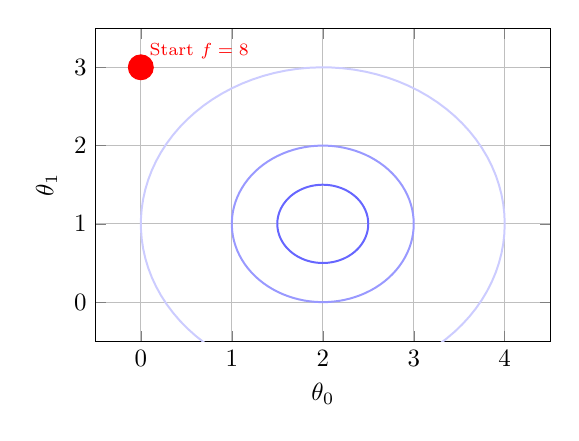
\begin{tikzpicture}[scale=0.9]
\begin{axis}[
    width=8cm, height=6cm,
    xlabel={$\theta_0$}, ylabel={$\theta_1$},
    xmin=-0.5, xmax=4.5, ymin=-0.5, ymax=3.5,
    grid=major
]

% Contours
\addplot[domain=0:360, samples=100, blue!20, thick] ({2+2*cos(x)}, {1+2*sin(x)});
\addplot[domain=0:360, samples=100, blue!40, thick] ({2+1*cos(x)}, {1+1*sin(x)});
\addplot[domain=0:360, samples=100, blue!60, thick] ({2+0.5*cos(x)}, {1+0.5*sin(x)});

% Start
\addplot[only marks, mark=*, mark size=5pt, red] coordinates {(0,3)};
\node[above right, red] at (axis cs:0,3) {\scriptsize Start $f=8$};

\end{axis}
\end{tikzpicture}
\end{figure}
\end{frame}

%===========================
\begin{frame}{Coordinate Descent: Step 1}
\begin{figure}
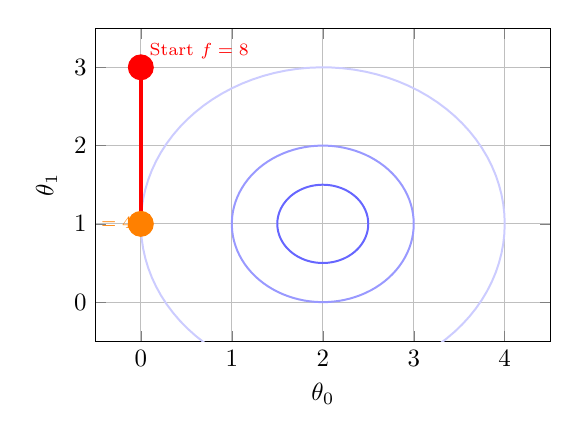
\begin{tikzpicture}[scale=0.9]
\begin{axis}[
    width=8cm, height=6cm,
    xlabel={$\theta_0$}, ylabel={$\theta_1$},
    xmin=-0.5, xmax=4.5, ymin=-0.5, ymax=3.5,
    grid=major
]

% Contours
\addplot[domain=0:360, samples=100, blue!20, thick] ({2+2*cos(x)}, {1+2*sin(x)});
\addplot[domain=0:360, samples=100, blue!40, thick] ({2+1*cos(x)}, {1+1*sin(x)});
\addplot[domain=0:360, samples=100, blue!60, thick] ({2+0.5*cos(x)}, {1+0.5*sin(x)});

% Start
\addplot[only marks, mark=*, mark size=5pt, red] coordinates {(0,3)};
\node[above right, red] at (axis cs:0,3) {\scriptsize Start $f=8$};

% Step 1
\addplot[->, ultra thick, red] coordinates {(0,3) (0,1)};
\addplot[only marks, mark=*, mark size=5pt, orange] coordinates {(0,1)};
\node[left, orange] at (axis cs:0,1) {\scriptsize Step 1: $f=4$};

\end{axis}
\end{tikzpicture}
\end{figure}
\end{frame}

%===========================
\begin{frame}{Coordinate Descent: Step 2}
\begin{figure}
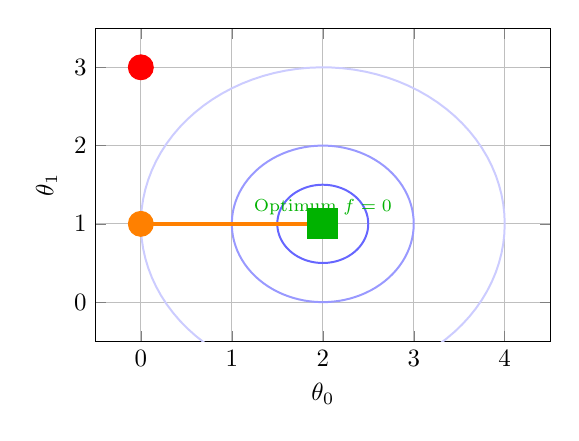
\begin{tikzpicture}[scale=0.9]
\begin{axis}[
    width=8cm, height=6cm,
    xlabel={$\theta_0$}, ylabel={$\theta_1$},
    xmin=-0.5, xmax=4.5, ymin=-0.5, ymax=3.5,
    grid=major
]

% Contours
\addplot[domain=0:360, samples=100, blue!20, thick] ({2+2*cos(x)}, {1+2*sin(x)});
\addplot[domain=0:360, samples=100, blue!40, thick] ({2+1*cos(x)}, {1+1*sin(x)});
\addplot[domain=0:360, samples=100, blue!60, thick] ({2+0.5*cos(x)}, {1+0.5*sin(x)});

% Start + Step 1
\addplot[only marks, mark=*, mark size=5pt, red] coordinates {(0,3)};
\addplot[only marks, mark=*, mark size=5pt, orange] coordinates {(0,1)};

% Step 2
\addplot[->, ultra thick, orange] coordinates {(0,1) (2,1)};
\addplot[only marks, mark=square*, mark size=6pt, green!70!black] coordinates {(2,1)};
\node[above, green!70!black] at (axis cs:2,1) {\scriptsize Optimum $f=0$};

\end{axis}
\end{tikzpicture}
\end{figure}
\end{frame}

\section{Failure of Coordinate Descent}

\section{Mathematical Derivation}

\begin{frame}{Lasso Coordinate Descent: Setup}
\begin{codebox}{Lasso Objective}
$$\text{Minimize } \sum_{i=1}^{n} (y_i - \hat{y}_i)^{2} + \lambda \sum_{j=0}^{d} |\theta_{j}|$$
\end{codebox}
\pause

\begin{keypointsbox}{Key Definitions}
\begin{itemize}
\item $\rho_j = \sum_{i=1}^{n} x_{ij}(y_i - \hat{y}_i^{(-j)})$ (partial residual correlation)
\item $z_j = \sum_{i=1}^{n} x_{ij}^2$ (feature norm squared)
\item $\hat{y}_i^{(-j)} = $ prediction without $j$-th feature
\end{itemize}
\end{keypointsbox}
\end{frame}

\begin{frame}{Lasso Coordinate Descent: Setup}
\begin{codebox}{Coordinate Update Rule}
Fix all $\theta_k$ for $k \neq j$, minimize w.r.t. $\theta_j$:
$$\min_{\theta_j} \sum_{i=1}^{n} (y_i - \hat{y}_i^{(-j)} - \theta_j x_{ij})^2 + \lambda |\theta_j|$$
\end{codebox}
\end{frame}

\begin{frame}{Subgradient Analysis}
\begin{codebox}{Subgradient of Lasso Objective w.r.t. $\theta_j$}
$$\frac{\partial}{\partial \theta_{j}}(\text{Lasso}) = -2\rho_{j} + 2\theta_{j}z_{j} + \lambda \frac{\partial}{\partial \theta_{j}}|\theta_{j}|$$
\end{codebox}
\pause

\begin{theorembox}{Subgradient of $|\theta_j|$}
$$\frac{\partial}{\partial \theta_{j}}|\theta_{j}| = \begin{cases}
+1 & \text{if } \theta_{j} > 0 \\
[-1,+1] & \text{if } \theta_{j} = 0 \\
-1 & \text{if } \theta_{j} < 0
\end{cases}$$
\end{theorembox}
\end{frame}

\begin{frame}{Soft-Thresholding Solution}
\begin{theorembox}{Complete Lasso Update Rule}
$$\theta_{j} = \begin{cases}
\frac{\rho_{j} + \lambda/2}{z_{j}} & \text{if } \rho_{j} < -\lambda/2 \\
0 & \text{if } |\rho_{j}| \leq \lambda/2 \\
\frac{\rho_{j} - \lambda/2}{z_{j}} & \text{if } \rho_{j} > \lambda/2
\end{cases}$$
\end{theorembox}

\begin{alertbox}{Sparsity Mechanism}
If correlation $|\rho_j| \leq \lambda/2$ is weak, set $\theta_j = 0$!
\end{alertbox}

\begin{keypointsbox}{Soft-Thresholding Properties}
{\small
\begin{itemize}
\item \textbf{Shrinkage}: Coefficients pulled toward zero
\item \textbf{Selection}: Small coefficients $\rightarrow$ exactly zero
\item \textbf{Smooth}: Continuous shrinkage + selection
\end{itemize}
}
\end{keypointsbox}
\end{frame}

\section{Lasso vs Ridge Comparison}

\begin{frame}{Lasso vs Ridge: Key Differences}
\begin{table}[h]
\centering
\begin{tabular}{|l|c|c|}
\hline
\textbf{Property} & \textbf{Ridge (L2)} & \textbf{Lasso (L1)} \\
\hline
Penalty & $\sum \theta_j^2$ & $\sum |\theta_j|$ \\
\hline
Sparsity & Never exactly zero & Can be exactly zero \\
\hline
Feature Selection & No & Yes \\
\hline
Differentiable & Yes & No (at $\theta_j = 0$) \\
\hline
Solution Method & Closed form & Coordinate descent \\
\hline
Constraint Shape & Circle & Diamond \\
\hline
Best for & Multicollinearity & Feature selection \\
\hline
\end{tabular}
\end{table}

\begin{keypointsbox}{When to Use Each}
{\small
\textbf{Lasso}: High-dimensional data, need interpretable model, expect few relevant features \\
\textbf{Ridge}: All features somewhat relevant, multicollinearity issues, want stable solution
}
\end{keypointsbox}
\end{frame}

\section{Summary and Applications}

\begin{frame}{Lasso Regression: Summary}
\begin{theorembox}{Three-Part Understanding}
\textbf{Visual}: L1 diamond constraint $\to$ sparsity at sharp corners \\
\textbf{Algorithmic}: Coordinate descent + soft-thresholding $\to$ exact zeros \\
\textbf{Mathematical}: Subgradients handle non-differentiability elegantly
\end{theorembox}

\begin{keypointsbox}{Key Advantages}
{\small
\begin{itemize}
\item Regression + feature selection simultaneously
\item Sparse, interpretable models
\item Handles high-dimensional data well
\end{itemize}
}
\end{keypointsbox}
\end{frame}

\begin{frame}{Lasso Regression: Summary}
\begin{keypointsbox}{Limitations}
{\small
\begin{itemize}
\item Arbitrary selection among correlated features
\item May underperform when all features are relevant
\end{itemize}
}
\end{keypointsbox}
\end{frame}

\begin{frame}{Applications and Extensions}
\begin{examplebox}{Real-World Applications}
{\small
\begin{itemize}
\item \textbf{Genomics}: 20,000+ genes $\to$ identify disease markers
\item \textbf{Text Mining}: 100k+ words $\to$ sentiment analysis features
\item \textbf{Signal Processing}: Sparse signal reconstruction
\item \textbf{Finance}: Risk factor selection from hundreds of indicators
\item \textbf{Marketing}: Customer segmentation with key attributes
\end{itemize}
}
\end{examplebox}

\begin{keypointsbox}{Extensions}
{\small
\begin{itemize}
\item \textbf{Elastic Net}: Combines L1 + L2 penalties
\item \textbf{Group Lasso}: Selects groups of related features
\item \textbf{Fused Lasso}: Enforces smoothness in ordered features
\end{itemize}
}
\end{keypointsbox}
\end{frame}

\end{document}